\documentclass{beamer}
%[aspectratio=169]   \usepackage[czech]{babel}
\usepackage{apo-lecture}
\usepackage{pdfpages}
\usepackage{pdfcomment}
\usepackage{listings}
\usepackage{array,multirow}
\usepackage{environ}

\subtitle{Lekce 09. Přerušení a události}
\author{Pavel Píša \phantom{xxxxxxxxx} Petr Štěpán \\ \small\texttt{pisa@fel.cvut.cz}\phantom{xxxx}\small\texttt{stepan@fel.cvut.cz}}

\begin{document}

\maketitle

\section{Oblasti využití počítačů/propojení s reálným světem}

\begin{frame}
\frametitle{Cíl dnešní přednášky}

\begin{itemize}
 \item Oblasti využití počítačů/propojení s reálným světem
 \item Obsluha periferií a vliv na zátěž procesoru
 \item Zpracování událostí, přerušení a výjimky
 \item Přímý přístup do paměti z periferií
 \item Konsekvence při použití skrytých pamětí, zpracování mimo pořadí, více procesorů
\end{itemize}
\end{frame}

\begin{frame}
\frametitle{Zopakování již probraných stavebních bloků}

\begin{itemize}
 \item Centrální procesorová jednotka
 \item Paměť/úložiště organizované do hierarchie
 \begin{itemize}
  \item zápisníková paměť (registry, rychlé)
  \item skrytá paměť (cache, úroveň L1, L2, ...)
  \item hlavní paměť (RAM -- dnes typicky DDR)
  \item vnější paměť, úložiště (disky, mžikové paměti -- Flash)
 \end{itemize}
 \item Propojení -- sběrnice, sítě
 \begin{itemize}
  \item ISA, PCI, PCIexpress, AXI
 \end{itemize}
\end{itemize}
\end{frame}

\begin{frame}
\frametitle{Oblasti, ve kterých lze bloky, procesory využít}

\begin{itemize}
 \item Zábava
 \begin{itemize}
  \item histricky první sekvenční stroje, automatofon - hrací skříňky, hodiny, orloje, mechanismus z Antikythéry již 150 př. n. l.
  \item dnes hrací automaty, herní konzole, simulátory, multimédia
 \end{itemize}
 \item Výdělečná zaneprázdněnost/aktivity (busyness)
 \begin{itemize}
  \item původně jen sčítačky, pokladny, dnes burzy cenných papírů, podnikové a bankovní informační systémy atd.
 \end{itemize}
 \item Rozsáhlé matematické, vědecké a modelovací výpočty
 \begin{itemize}
  \item globální klimatické prognózy a analýzy, jaderná fúze atd
  \item strojové učení
 \end{itemize}
 \item Komunikace
 \begin{itemize}
  \item jako hlavní cíl síťové prvky, původně telefon pevný, mobilní
  \item dnes součást téměř všech ostatních aplikací
 \end{itemize}
 \item Automatizace, výroby, dopravy
 \begin{itemize}
  \item původně automatické vzory tkalcovský stav, dnes sváření, robotika, autonomní automobily a vlaky
 \end{itemize}
 \item a mnoho dalších oblastí
\end{itemize}
\end{frame}

\begin{frame}
\frametitle{Počítač v řídicích aplikacích}

\begin{columns}
\begin{column}{0.58\textwidth}
Nahrazuje na míru sestavené regulátory. Výhody:
\begin{enumerate}
 \item často složitý řídicí proces, pravidla, vztahy
 \begin{itemize}
   \item rychlý výpočet
 \end{itemize}
 \item levný díky sériové výrobě
 \item velmi flexibilní
 \begin{itemize}
   \item programování
 \end{itemize}
 \item snadná realizace hierarchického řízení
 \begin{itemize}
   \item ovládání k dispozici
 \end{itemize}
 \item přesné/deterministické zpracování veličin
 \begin{itemize}
   \item zobrazení hodnot a jeho limity 
 \end{itemize}
 \item komplexní algoritmy
 \begin{itemize}
   \item pouze paměťová a časová omezení
 \end{itemize}
\end{enumerate}
  \vfil
\end{column}
\begin{column}{0.42\textwidth}
  \begin{center}
    Počítač jako řídící systém

    \vspace{5mm}

    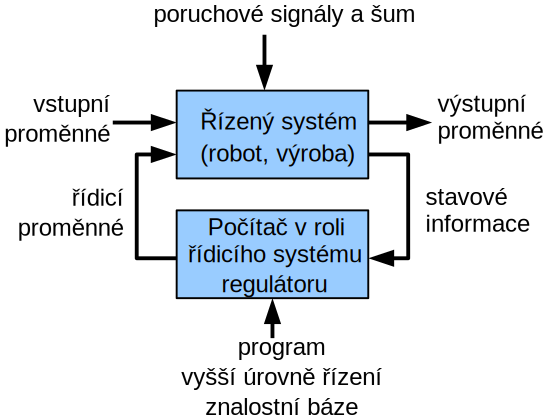
\includegraphics[width=1.0\textwidth]{computer-as-controller-cz.pdf}
  \end{center}
\end{column}
\end{columns}
\end{frame}

\begin{frame}
\frametitle{Různé požadavky na zpracování úloh, dat}

\begin{itemize}
 \item Dávkové zpracování
 \begin{itemize}
  \item úloha řídí přístupy k datům podle toho, jak je potřebuje zpracovávat, stejně tak časování a pořadí uložení výstupů se řídí potřebami výpočtu
 \end{itemize}
 \item Interaktivní
 \begin{itemize}
  \item obvykle událostmi řízené v kombinaci podle požadavků, vstupů od uživatele nebo z jiného systému
 \end{itemize}
 \item Řízení (technologií, robotů, automobilů) v reálném čase
 \begin{itemize}
  \item sebepřesnější výstupy dodané pozdě nemají žádnou hodnotu (letadlo již havarovalo) nebo výrazně sníženou (nespojitý přenos videa)
  \item stupeň integrity bezpečnosti (Safety Integrity Level -- SIL) pokud hrozí újma na zdraví a majetku
 \end{itemize}

\end{itemize}
\end{frame}

\section{Obsluha periferií}

\begin{frame}
\frametitle{Vstupně-výstupní subsystém (opakování)}

\begin{itemize}
 \item Periferie pouze pro vstup
 \begin{itemize}
  \item  běžné: klávesnice, myš, videokamera
  \item digitální vstupy, fyzikální veličiny -- obvykle převedeny na analogové
elektrickým signálem a následně A/D převodníkem na číselnou hodnotu
přístupné na vstupním portu a dalších senzorech
 \end{itemize}
\end{itemize}
\begin{itemize}
 \item Pouze výstupné periferií
 \begin{itemize}
  \item video výstup (2D, 3D + akcelerace), audio výstup
  \item výstupy s fyzickým efektem, 3D tiskárna (rychlé prototypování),
řízení technologických procesů (D/A převodníky, PWM) a mnohé
jiné druhy pohonů
 \end{itemize}
\end{itemize}
\begin{itemize}
 \item Obousměrná komunikace
 \begin{itemize}
  \item pevný disk, komunikační rozhraní
  \item většina výše uvedených „jednosměrných“ periferií vyžaduje čtení
a přístup pro zápis pro jejich nastavení, monitorování a parametry
řízení
 \end{itemize}
\end{itemize}
\end{frame}

\begin{frame}
\frametitle{Metody přenosu dat mezi periferiemi a procesorem}

\begin{itemize}
 \item Programovaný vstup/výstup s dotazováním (anglicky programmed input/output -- PIO with polling)
 \begin{itemize}
  \item procesor se cyklicky dotazuje na stavové informace periferie
        jestli jsou dostupná vstupní data nebo místo ve výstupní vyrovnávací paměti
 \end{itemize}
\end{itemize}
\begin{itemize}
 \item Programovaný vstup/výstup řízený přerušením (anglicky programmed input/output PIO)
 \begin{itemize}
  \item procesor/program/operační systém konfiguruje periferie, ale nečeká
        na data. Příchod dat je signalizován přerušením (asynchronní
        událost/výjimka). Data jsou čtena v obslužné rutině přerušení (interrupt service routine -- ISR).
 \end{itemize}
\end{itemize}
\begin{itemize}
 \item Přímý přístup do paměti (anglicky direct memory access -- DMA)
 \begin{itemize}
  \item procesor/program/operační systém nastaví zdroj a cíl, přenos realizuje
        specializovaná jednotka, dokončení signalizované přerušením.
 \end{itemize}
\end{itemize}
\begin{itemize}
 \item Inteligentní periferie/řadiče 
 \begin{itemize}
  \item realizující operaci i s přenosem do paměti (bus master -- DMA)
 \end{itemize}
\end{itemize}
\end{frame}

\section{Zpracování událostí, přerušení a výjimky}

\begin{frame}
\frametitle{Základní cyklus procesoru (opakování z lekce 2)}
\begin{enumerate}
  \item Počáteční nastavení -- inicializace registru PC a PSW (případně i dalších) po zapnutí proudu nebo po resetu procesoru
  \item Přečti instrukci z paměti z adresy PC
  \begin{itemize}
    \item nastav PC na adresu sběrnice paměti
    \item Přečti obsah ze sběrnice paměti do registru IR
    \item $PC+l \to PC$, uprav $PC$, $l$ je délka načtené instrukce
  \end{itemize}
  \item Dekóduj instrukci
  \item Proveď instrukci
  \begin{itemize}
    \item spočti adresu, vyber registry, načti operandy, proveď požadovaný výpočet ALU a ulož výsledky
  \end{itemize}
  \item \textbf{Zkontroluj zda není přerušení nebo výjimka}
  \begin{itemize}
    \item pokud je výjimka důsledkem vykonávání dané instrukce, zajisti, že její výstupy nejsou uloženy a $PC$ na ní dále ukazuje
    \item přejdi na obslužnou rutinu tak, aby bylo možné po návratu v přerušené sekvenci instrukcí pokračovat
  \end{itemize}
  \item Opakuj od kroku 2
\end{enumerate}
\end{frame}

\begin{frame}
\frametitle{Výjimky a přerušení}

\begin{itemize}
 \item Výjimky (synchronní) -- anomální nebo výjimečné situace znemožňují pokračování běhu sekvence instrukcí a vyžadující zvláštní zpracování, hlavní uvažované zdroje
 \begin{itemize}
  \item nedefinovaná instrukce (RISC V -- neznámý operační kód -- unknown opcode)
  \item aritmetická výjimka (dělení nulou, přetečení -- na RISC-V neexistuje pro celočíselnou jednotku, pro plovoucí řádovou čárku ano)
  \item systémové volání (vyvolává instrukce systémového volání -- syscall)
  \item data nejsou dostupná nebo došlo k chybě čtení/zápisu
  \item chyba v adrese, stránka označená jako neplatná, chráněný rozsah atd.
  \item nedovolená instrukce pro daný režim procesoru (uživatelský, systémový, strojový)
  \item byla zjištěna chyba sběrnice (parita, kontroly a opravy chyb -- ECC, překročen čas na potvrzení)
 \end{itemize}
 \item Asynchronní/externí výjimky (přerušení)
 \begin{itemize}
  \item nejsou přímým důsledkem vykonání dané aktuální instrukce
  \item většinou nelze určit na instrukci, hodinový cyklus, přesně, kdy k~události dojde
 \end{itemize}
\end{itemize}
\end{frame}

\begin{frame}
\frametitle{Asynchronní/externí výjimky (přerušení)}

\begin{itemize}
 \item maskovatelné, lze zakázat ve stavovém/řídicím slovu procesoru (processor status word -- PSW)
 \begin{itemize}
   \item buď všechna nebo do určité priority zdroje
   \item periferní zařízení, čítače, časovače
   \item meziprocesorová komunikace, notifikace dalších jader, že mají převzít úlohu a další
   \item většinou i na vlastním zdroji nebo řadiči povolení a volitelně i nastavení priority
 \end{itemize}
 \item nemaskovatelné
 \begin{itemize}
  \item poruchy hardware, dohledové obvody (Watch Dog)
 \end{itemize}
\end{itemize}
\end{frame}

\begin{frame}
\frametitle{Kroky při zpracování výjimek nebo přerušení}

\begin{itemize}
 \item Výjimka se přijímá/zpracovává obvykle bezpodmínečně,
externí přerušení pouze tehdy, není-li maskováno nebo není-li maskováno
\end{itemize}

\begin{enumerate}
 \item Vektor stavu procesoru je uložen včetně čítače instrukcí ($PC$)
 \begin{itemize}
  \item na systémový zásobník a nebo do specializovaných registrů procesoru (ELR, EPC)
  \item kolik je uloženo již v první fázi hardwarem a kolik později obslužnou rutinou se mezi architekturami liší
  \item při přerušení běhu v uživatelském režimu je režim přepnutý na systémový nebo strojový (machine)
  \item obvykle další přerušení nebo nižší a rovné priority jsou zakázané
 \end{itemize}
 \item Čítač instrukcí je přednastaven na počáteční adresu obslužné rutiny
 \begin{itemize}
  \item buď jedné pro všechny zdroje, případně podle typu výjimky nebo i jednotlivého čísla zdroje přerušení
 \end{itemize}
 \item Provede se servisní rutina začínající na této adrese
 \begin{itemize}
  \item ta ukládá obvykle stav ostatních ohrožených registrů na zásobník, komunikuje s periferiemi,
        načte chybějící stránku, informuje o neobnovitelné chybě úlohy nebo celého systému atd.
 \end{itemize}
\end{enumerate}
\end{frame}

\begin{frame}
\frametitle{roky při zpracování výjimek nebo přerušení -- ukončení obsluhy}

\begin{enumerate}
 \setcounter{enumi}{4}
 \item Spadá-li důvod mezi obnovitelné zdroje (recoverable) -- obnoví rutina hodnoty registrů do stavu před spuštěním
 \item Rutina je dokončena speciální instrukcí návratu výjimky
 \begin{itemize}
  \item tím doje přepnutí procesoru do předchozího stavu včetně čítače instrukcí a umožní tak pokračování
        přerušeného kódu
 \end{itemize}
\end{enumerate}
\begin{itemize}
 \item Dále již pokračuje buď zopakování instrukce, která výjimku způsobila, nebo se pokračuje od další instrukce,
       případ externího přerušení, systémového volání nebo emulace instrukce, která není přímo podporovaná
\end{itemize}
\end{frame}

\begin{frame}
\frametitle{Zdroje výjimek na architektuře RISC-V}

\begin{itemize}
 \item Výjimky způsobené poruchou hardwaru:
 \begin{itemize}
  \item kontrola stroje (Machine Check): Procesor detekuje vnitřní nekonzistenci
  \item chyba sběrnice (Bus Error): při načtení nebo uložení instrukce nebo načtení instrukce
 \end{itemize}
 \item Výjimky způsobené některými vnějšími příčinami (pro procesor):
 \begin{itemize}
  \item znovunastavení (Reset): Signál aktivovaný na příslušném vývodu pouzdra, jádra
  \item nemaskovatelné přerušení (NMI): Náběžná hrana signálu NMI na příslušném signálu
 \end{itemize}
 \item Hardwarová přerušení: Aktivovaná příslušnými signály
 \begin{itemize}
  \item hardwarová přerušení lze maskovat nastavením příslušných bitů stavového registru
 \end{itemize}
 \item Výjimky, které se vyskytují v důsledku problémů s vykonáním instrukce
\end{itemize}
\end{frame}

\begin{frame}
\frametitle{Zdroje výjimek na architektuře RISC-V -- pokračování}

\begin{itemize}
 \item Výjimky, které se vyskytují v důsledku problémů s vykonáním instrukce
 \begin{itemize}
  \item chyba v adrese (Address Error): odkaz na neplatnou oblast paměti, popř.
odkaz na adresní prostor jádra z uživatelského režimu
 \item neplatná instrukce: Nedefinované pole operačního kódu (nebo privilegované
instrukce v uživatelském režimu)
 \end{itemize}
 \item Výjimky způsobené prováděním k tomu určených instrukcí
 \begin{itemize}
  \item systémové volání (Syscall): Provedená instrukce \textbf{ecall}
  \item instrukce pozastavení (Break): Provedená instrukce \textbf{ebreak}
 \end{itemize}
\end{itemize}
\end{frame}

\begin{frame}
\frametitle{RISC-V -- stavové a řídicí registry pro obsluhu výjimek}

\begin{tabular}{|l|l|l|}  \hline
Jméno registru & Číslo & Význam/využití \\\hline
mstatus & 0x300 & Machine status register \\\hline
misa & 0x301 & ISA and extensions \\\hline
mie & 0x304 & Machine interrupt-enable register \\\hline
mtvec & 0x305 & Machine trap-handler base address \\\hline
mscratch & 0x340 &Scratch register for machine trap handlers \\\hline
mepc & 0x341 & Machine exception program counter \\\hline
mcause & 0x342 & Machine trap cause \\\hline
mtval &0x343 & Machine bad address or instruction \\\hline
mip & 0x344 & Machine interrupt pending \\\hline
mtinst & 0x34A & Machine trap instruction (transformed) \\\hline
\end{tabular} 

\vspace{3mm}

The RISC-V Instruction Set Manual – Volume II: Privileged Architecture

\url{https://riscv.org/technical/specifications/}
\end{frame}

\begin{frame}
\frametitle{RISC-V -- stavový registr v 32-bitové variantě}

Machine Status Register -- \textbf{mstatus} (RV32)

\begin{center}
  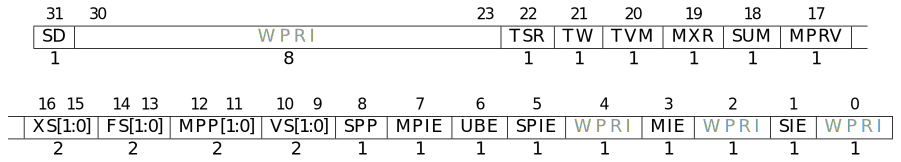
\includegraphics[width=0.95\textwidth]{riscv-mstatus.pdf}
\end{center}

\begin{tabular}{|l|l|l|}  \hline
Pole & Bit(y) & Význam/využití \\\hline
SIE & 1 & Supervisor global interrupt enable \\\hline
MIE & 3 & Machine global interrupt enable (for handler atomicity) \\\hline
SPIE & 5 & SIE before trapping to system mode \\\hline
MPIE & 7 & MIE before trapping to machine mode \\\hline
SPP & 8 & Priority mode before trapping to system mode \\\hline
VS & 10:9 & Inform if floating point save is needed \\\hline
MPP & 12:11 & Priority before trapping into machine mode \\\hline
\end{tabular}
\end{frame}

\begin{frame}
\frametitle{RISC-V -- registr příčiny výjimky/přerušení}

Machine Cause Register (mcause) -- \textbf{mstatus}

\begin{center}
  
\includegraphics[width=0.95\textwidth]{riscv-mcause.pdf}
\end{center}

\small
Registr informuje obslužnou rutinu o zdroji výjimky, přerušení.

Pokud je nastavený nejvýznamnější bit (RV32 bit 31, RV64 bit 63), pak je zdroj
asynchronní výjimka/periferní/externí přerušení. Kód výjimky odpovídá
zdroji a odpovídající pozici bitu povolení a nevyřízeného zdroje v registrech
\textbf{mie} a \textbf{mip}. \textbf{mepc} ukazuje na přerušenou (první nezpracovanou)
instrukci. Návrat jednoduše instrukcí \textbf{mret} bude pokračovat v provádění přerušeného
programu od~další instrukce. Když je nejvýznamnější bit nulový, jedná se o synchronní zdroj výjimky.
\textbf{mepc} ukazuje na instrukci která jí způsobila. Pokud je příčina
(např. výpadek stránky) vyřešena, instrukci bude znova spuštěná jednoduše
po návratu \textbf{mret}. Pokud je důvodem systémové volání (instrukce ecall), \textbf{ebreak} popř.
neplatná instrukce, která je emulována obsluhou, pak je nutné \textbf{mepc} před návratem \textbf{mret}
posunout za instrukci, která výjimku způsobila.


\end{frame}

\begin{frame}
\frametitle{RISC-V -- kódování příčin synchronních výjimek}

\begin{center}
\small
\begin{tabular}{|l|l|l|}  \hline
Vnější (IRQ) & Číslo & Důvod/zdroj \\\hline
0 & 0 &Instruction address misaligned \\\hline
0 & 1 & Instruction access fault \\\hline
0 & 2 & Illegal instruction \\\hline
0 & 3 & Breakpoint exception \\\hline
0 & 4 & Load address misaligned \\\hline
0 & 5 & Load access fault \\\hline
0 & 6 & Store/AMO address misaligned \\\hline
0 & 7 & Store/AMO access fault \\\hline
0 & 8 & Environment call from U-mode \\\hline
0 & 9 & Environment call from S-mode \\\hline
0 & 11 & Environment call from M-mode \\\hline
0 & 12 & Instruction page fault \\\hline
0 & 13 & Load page fault \\\hline
0 & 15 & Store/AMO page fault \\\hline
0 & 24...31 &Designated for custom use \\\hline
\end{tabular}
\end{center}
\end{frame}

\begin{frame}
\frametitle{RISC-V -- kódování příčin asynchronních přerušení}

\begin{center}
\small
\begin{tabular}{|l|l|l|}  \hline
Vnější (IRQ) & Číslo & Důvod/zdroj \\\hline
1 & 1 & Supervisor software interrupt \\\hline
1 & 3 & Machine software interrupt \\\hline
1 & 5 & Supervisor timer interrupt \\\hline
1 & 7 & Machine timer interrupt \\\hline
1 & 9 & Supervisor external interrupt \\\hline
1 & 11 & Machine external interrupt \\\hline
1 & ≥16  & Designated for platform use \\\hline
\end{tabular}
\end{center}

\small
Registr \textbf{mie} povoluje jednotlivé zdroje přerušení, pozice bitu odpovídá
zdroji

Registr \textbf{mip} informuje o aktuálně čekajících/nevyřízených zdrojích

\textbf{mstatus.MIE} globální povolení (1) / zakázání (0)

Existuje další sada registrů pro úroveň systému
kontrola

\textbf{sstatus}, \textbf{sie}, \textbf{sip}, \textbf{sscratch}, \textbf{scause} atd. Jejich struktura je
stejná/podobná, ale jsou přístupné z režimu systému (supervisor), kdy ovládání na úrovni stroje (machine) není povoleno
\end{frame}

\begin{frame}
\frametitle{RISC-V -- zpracování výjimek a přerušení}

Procesor přijme přerušení, výjimku nebo \textbf{ecall} operační znak (ten v režimu uživatele, systému, stroje)

\begin{itemize}
 \item mepc <= pc and switches to machine privilege mode
 \item mstatus.MPP and mstatus.MPV set to preceding privilege mode
 \item mcause <= exception code, mcause[XLEN-1] <= 1 if interrupt
 \item mstatus.MPIE <= mstatus.MIE, mstatus.MIE <= 0
 \item PC <= mtvec (for vectored mode and interrupts BASE+4×cause)
\end{itemize}

Počátek, prolog, obslužné rutiny je zodpovědný za zjištění příčiny \texttt{csrr rd, mcause}

Stav procesoru je sledovaný a řízený přes kontrolní a stavové registry (control an status registers -- CSR)

\begin{tabular}{l r l}
\multicolumn{2}{l}{\texttt{csrrw rd, csr, rs1}} & \texttt{csrrwi rd, csr, uimm5} \\
\multicolumn{2}{l}{\texttt{csrr(s/c)(i) rd, csr, rs1}}  & \texttt{csrr(s/c)(i) rd, csr, uimm5} \\
\texttt{csrr rd, csr} &  odpovídá  & \texttt{csrrs rd, csr, x0} \\
\texttt{csrw csr, rs} &  odpovídá  & \texttt{csrrw x0, csr, rs1} \\
\end{tabular}
\end{frame}

\begin{frame}
\frametitle{RISC-V -- zakončení zpracování výjimek a přerušení}

Obslužná rutina informuje instrukcí \textbf{mret} (ze systémového režimu \textbf{sret})
o~ukončení obsluhy výjimky/přerušení a procesor provede přepnutí do uloženého, obvykle původního
režimu a programu

\begin{itemize}
 \item priviledge mode from mstatus.MPP and mstatus.MPV
 \item mstatus.MPV <= 0, mstatus.MPP <= 0
 \item mstatus.MIE <= mstatus.MPIE
 \item pc <= mepc and continue execution in mode restored from mstatus.MPP
\end{itemize}
\end{frame}

\begin{frame}
\frametitle{Precizní obsluha výjimek}

Pokud je přerušení/výjimka úspěšně zpracována (tj. chybí
stránka byla zaměněna atd.) tak provádění pokračuje
instrukcí, která ho způsobila (na které byla výjimka přijata).
Tok přerušeného kódu se nezmění a~z~pohledu programu nelze
detekovat, že problému došlo (kromě zpoždění/časování a případů,
kdy je modifikace  stavu zamýšlena/způsobena obsluhou systémových
volání)

\vspace{3mm}

Poznámka: Přesné zpracování výjimek je nejvíce komplikované
zpožděnými zápisy (změna pořadí vykonávání instrukcí na superskalárních architekturách).
To vede k detekci synchronních výjimek i o mnoho
instrukcí později. Koncept obnovení stavu (rollback) nebo
potvrzení „transakcí“ je pak nutný pro zajištění stránkování paměti atd.
\end{frame}

\begin{frame}
\frametitle{Varianty vyhodnocení zdrojů výjimek}

\begin{itemize}
 \item Softwarové vyhodnocení příčiny
 \begin{itemize}
  \item Obsluha vyhodnocení všech výjimek/přerušení začíná stejnou rutinou na stejné adrese --
        tj. pro RISC-V je $PC$ nastavena na hodnotu \textbf{mtvec}. Pro systémový režim \textbf{stvec}.
  \item Rutina čte zdroj ze stavového registru (RISC-V: \textbf{mcause} Registrovat)
 \end{itemize}
 \item Vektorové zpracování výjimek (na RISC-V se většinou nepoužívá)
 \begin{itemize}
  \item Identifikace zdroje příčiny v příčiny/zdroj/čísla přerušení v hardware procesoru
  \item Pole počáteční adres obslužných rutin je vyplněno na pevné nebo přednastavené adrese
  (VBR -- bázový registr tabulky) v hlavní paměti
  \item CPU vypočítá index do tabulky na základě čísla zdroje
  \item CPU načte slovo z dané adresy do PC
 \end{itemize}
 \item Nevektorové zpracování výjimek s více rutinami/počátkem
       adresy přiřazené třídám výjimek a nebo prioritám přerušení
\end{itemize}

\footnotesize

Na RISC-V buď čistě softwarově, rutina od~\textbf{mtvec} nebo když \textbf{mtvec}.0=1, tak \textbf{mtvec} ukazuje na tabulku,
pak na pozici nula odkaz na obsluhu (vnějších) přerušení, a dále položky pro jednotlivé synchronní výjimky.
\end{frame}

\begin{frame}[fragile]
\frametitle{Příklad obsluhy přerušení -- počáteční nastavení}

\begin{columns}
\begin{column}{0.5\textwidth}
\begin{minted}[fontsize=\footnotesize]{gas}
_start:
   addi   a0, zero, 0x101
   la     t0, skip
   csrrw  zero, mepc, t0
   mret   # test exception ret
   addi   a0, zero, 0x105
   addi   a0, zero, 0x106
skip:
   addi   a0, zero, 0x107
   csrrs  t0, mepc, zero
   ebreak
   la     t0, handle_exception
   csrrw zero, mtvec, t0
   la     t0, task_control_block
   csrrw zero, mscratch, t0
   csrrsi zero,mstatus,8 # MIE=1
   addi t0, zero, 16 # UART RX
   addi t1, zero, 1
   sll t1, t1, t0 # bit mask
\end{minted}
\end{column}
\begin{column}{0.5\textwidth}
\begin{minted}[fontsize=\footnotesize]{gas}
   csrrs zero, mie, t1
   li   a0, SERIAL_PORT_BASE
   li   t0, SERP_RX_ST_REG_IE_m
   sw   t0, SERP_RX_ST_REG_o(a0)
   # Background task
   addi t0, zero, 0x0001
   li   a0, SPILED_REG_BASE
Loop:
   csrrs t1, mepc, zero # check
   sw   t1,SPILED_REG_LED_LINE(a0)
   srl t2, t0, 31
   sll t0, t0, 1
   or   t0, t0, t2
   lw   t2, ..._KNOBS_8BIT(a0)
   sw   t2, ..._LED_RGB1(a0)
   xori t2, t2, -1
   sw   t2, ..._LED_RGB2(a0)
   beq zero, zero, loop
\end{minted}
\end{column}
\end{columns}

\end{frame}

\begin{frame}[fragile]
\frametitle{Příklad obsluhy přerušení -- obslužná rutina}

\begin{minted}[fontsize=\footnotesize]{gas}
handle_exception:
    csrrw   tp, mscratch, tp      # store previous and take system tp
    sw      sp, TCB_SP(tp)        # store stack pointer
    sw      ra, TCB_RA(tp)        # store return address
    sw      t0, TCB_T0(tp)        # store rest of clobberable regs
    sw      a0, TCB_A0(tp)
    ...
    csrr    t0, mcause            # is it Rx interrupt?
    blt     t0, zero, handle_irq  # branch to interrupts processing
    ...
    # handle synchronous exception
ret_from_exception:
    lw      sp, TCB_SP(tp)        # restore stack pointer
    lw      ra, TCB_RA(tp)        # restore return address
    lw      t0, TCB_T0(tp)        # restore rest of clobberable regs
    lw      a0, TCB_A0(tp)
    ...
    csrrw   tp, mscratch, tp      # Swap back TCB to mscratch
    mret                          # Return from exception pc <= mepc
\end{minted}
\end{frame}

\begin{frame}[fragile]
\frametitle{Příklad obsluhy přerušení -- obsluha sériového portu}

\begin{minted}[fontsize=\footnotesize]{gas}
handle_irq:                        # t0 mcause
    slli    t0, t0, 2              # shift out sign, left sources * 4
    # the t0 would be used to point into irq handlers table
    # check only for UART RX interrupt for simplicity 8
    addi    a0, zero, 16 * 4       # UART RX is the first platform irq
    beq     t0, a0, handle_uart_rx_irq # it is UART RX
    # mask out unknown sources
    srli    t0, t0, 2              # make t0 back simple source index
    addi    a0, zero, 1
    sll     a0, a0, t0             # generate bit mask for source
    csrrc   zero, mie, a0          # mie = mie & ~a0
    j       ret_from_exception
handle_uart_rx_irq:
    li      a0, SERIAL_PORT_BASE   # Setup base of UART
    lw      t0, SERP_RX_DATA_REG_o(a0) # Read received character
    sw      t0, SERP_TX_DATA_REG_o(a0) # echo it back to terminal
    j       ret_from_exception
\end{minted}

\tiny

\url{https://gitlab.fel.cvut.cz/b35apo/stud-support/-/blob/master/seminaries/qtrvsim/uart-echo-irq/uart-echo-irq.S}

QtRVSim simulátor v RISC-V zatím podporu nemá, QtMips, v MIPS přerušení podporuje.

\end{frame}

\begin{frame}
\frametitle{Přerušení k obsluze V/V v operačním systému}

Když aplikace čeká na příchozí data nebo na prostor na odeslání dalších, tak je úloha pozastavena/čeká (procesor může obsluhovat jinou úlohu).
Periferie po přijetí dat informuje procesor přerušením a ten dokončí přenos a uvolní původní úlohu pokračování

\begin{center}
  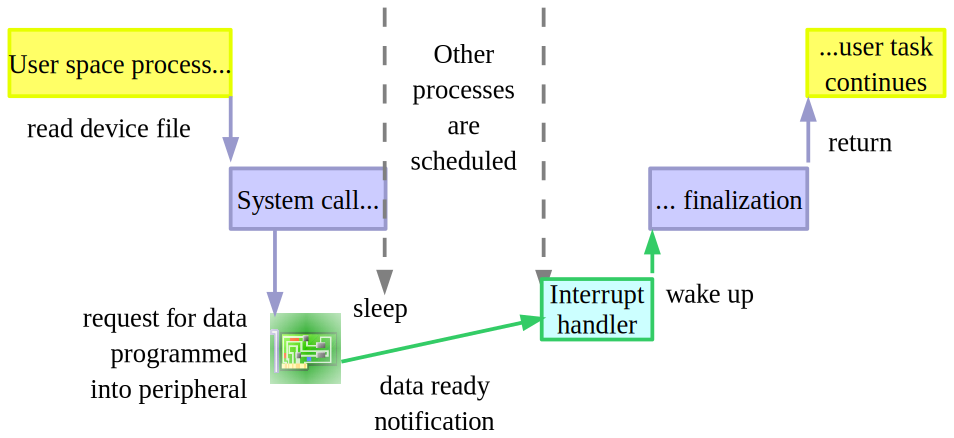
\includegraphics[width=0.95\textwidth]{irq-and-os-intercation.pdf}
\end{center}

\tiny

Zdroj: bootlin: Kernel, drivers and embedded Linux development \url{https://bootlin.com/}

\end{frame}

\section{Přímý přístup do paměti z periferií (DMA)}

\begin{frame}
\frametitle{Přímý přístup do paměti z periferií}

\begin{itemize}
 \item Procesor nastaví periferii a adresu do paměti odkud/kam mají být data přenesena
 \item Poté je spuštěný přenos a buď přímo periferie provádí přístupy do hlavní paměti
       a nebo přes požadavek žádá obecný řadič přímých přenosů (DMA controller)
 \item Klasických sdílených sběrnic je nutné zajistit, že pro každý datový přenos, cyklus
       sběrnice dojde uvolnění řízení sběrnice centrálním prvkem, procesorem a volbu adresy
       a řízení přenosu dat provádí periferie případně obecný řadič
 \item Po přenesení nastaveného počtu bytů dojde k informaci procesoru o dokončení přenosu
       nebo o přípdané chybě mechanizmem vyvolání přerušení
\end{itemize}

\end{frame}

\begin{frame}
\frametitle{Přímý přístup do paměti -- čtení z disku, krok 1}

\begin{center}
  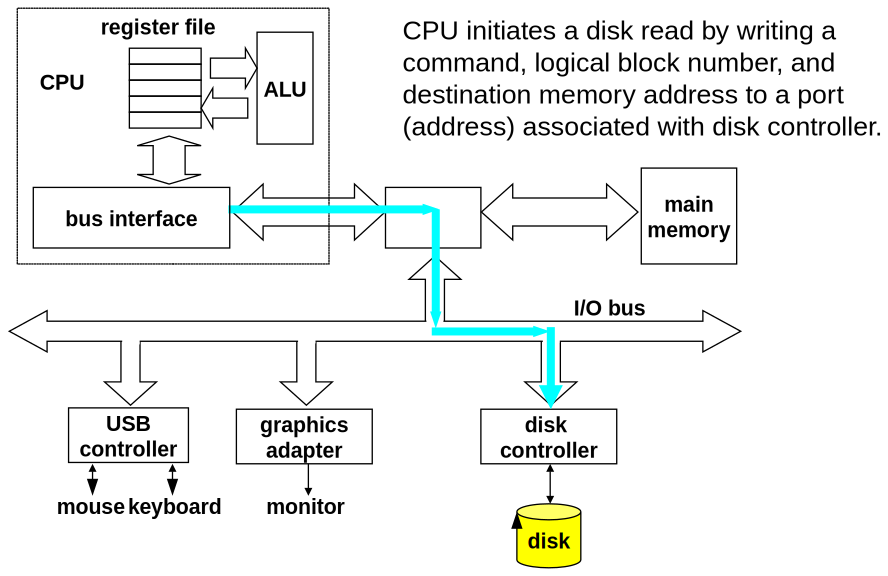
\includegraphics[width=0.90\textwidth]{dma-transfer-1.pdf}
\end{center}

\end{frame}


\begin{frame}
\frametitle{Přímý přístup do paměti -- čtení z disku, krok 2}

\begin{center}
  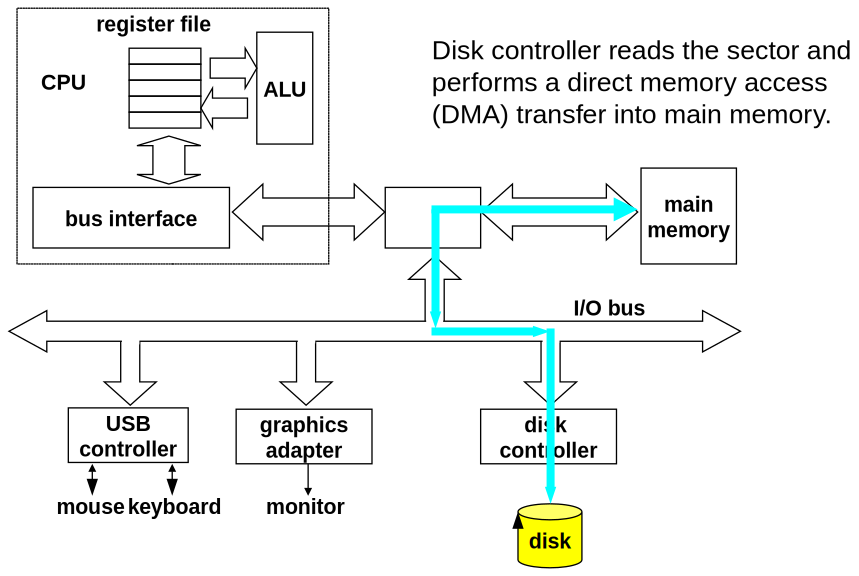
\includegraphics[width=0.90\textwidth]{dma-transfer-2.pdf}
\end{center}

\end{frame}

\begin{frame}
\frametitle{Přímý přístup do paměti -- čtení z disku, krok 3}

\begin{center}
  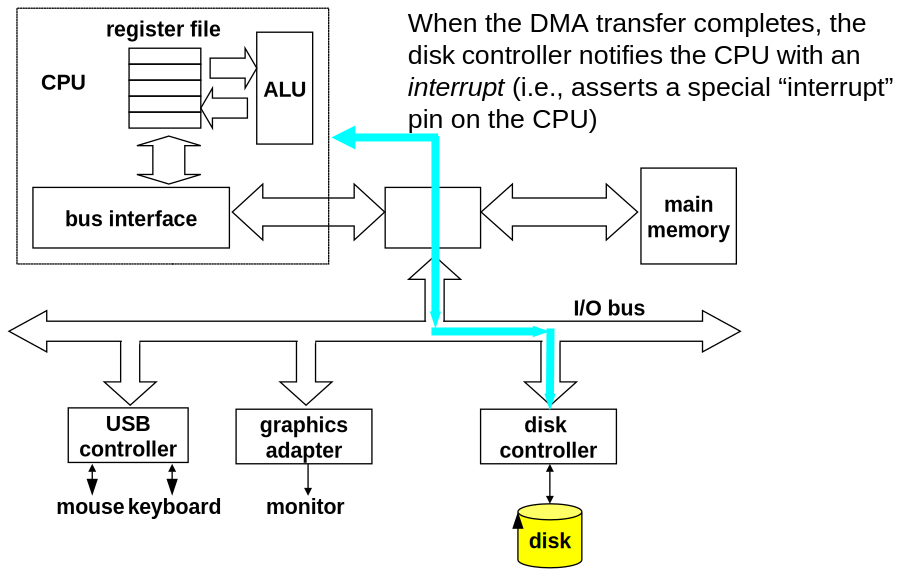
\includegraphics[width=0.90\textwidth]{dma-transfer-3.pdf}
\end{center}

\end{frame}

\section{Konsekvence při použití skrytých pamětí, zpracování mimo pořadí, více procesorů}

\begin{frame}
\frametitle{Skryté paměti, více procesorů a nebo přístupy z periferií}

\begin{itemize}
 \item Při přístupu k paměti mimo dané procesorové jádro je nutné počítat s tím, že data se mohou
       nacházet ve skrytých pamětech (cache) na různých úrovních paměťové hierarchie
 \item Přístup bez zneplatnění nebo obnovení povede k porušen podmínek paměťové koherence
 \item O tu se pro většinu víceprocesorových/jádrových systémů minimálně mezi vlákny
       stará hardware procesoru
 \item Koherence s přenosy z periferií je na různých architekturách a jejich implementacích
       řešena různě, obecně platí, že operační systém má volat pro oblasti určené pro
       pro příjem a vyslání dat před předáním periferii funkce, které se o synchronizaci
       nebo zneplatnění oblasti ve skrytých pamětech, pokud je to potřeba postarají
\end{itemize}
\end{frame}

\begin{frame}[fragile]
\frametitle{Vykonávání instrukcí mimo pořadí a paměťové bariéry}

\begin{itemize}
 \item Budeme předpokládat, že koherence jednotlivých lokací v paměti je vyřešená, ať v hardware nebo pro periferie softwarově
 \item Pokud však procesor vykonává instrukce mimo pořadí, tak i přístupy do paměti mohou pořadí měnit
 \item Může se stát, že například instrukce pro spuštění přenosu zapíše data dříve, než je nastavená cílová adresa
 \item Stejně tak může vláknu na druhém procesoru potvrdit zápisem do paměti, že jsou na jiné adrese data připravená,
       ale instrukce zápisů nejsou dokončené
 \item I kompilátor může libovolně přeorganizovat pořadí přístupů nebo opakované vynechat
\end{itemize}

\end{frame}

\begin{frame}[fragile]
\frametitle{Vykonávání instrukcí mimo pořadí  a paměťové bariéry}

\begin{itemize}
 \item Je tedy nutné definovat sekvenční body přes které se žádné nebo jen určité přístupy v čase
       dopředu a dále nepřesouvají. K tomu slouží pro každý jazyk, běhové prostředí definované
       konstrukce a na úrovni procesoru pak specializované instrukce. Na MIPS například \textbf{sync}, na RISC-V \textbf{fence}
       na x86 přetížené historické instrukce. Pro x86 vyvolání bariéry z GCC
\end{itemize}

\begin{minted}[fontsize=\footnotesize]{c}
__asm__ volatile ("xchgl %0,%1" :"=r" (x) :"m" (y), "0" (x) :"memory");
\end{minted}
\end{frame}

\end{document}

